% =====================================================================
%  Proposal presentation (Beamer, single-file) — PRIMARY track
%  Inter-Animal Mask-Contact Geometry for Social Behaviour Recognition
%  Build:  ../build.sh presentation     (Tectonic + Ghostscript-normalise)
% =====================================================================
\documentclass[aspectratio=169,11pt]{beamer}
\usetheme{default}
\setbeamertemplate{navigation symbols}{}
\setbeamertemplate{footline}[frame number]
\setbeamertemplate{itemize items}[circle]

\usepackage{amsmath}
\usepackage{tikz}
\usetikzlibrary{positioning,arrows.meta,calc}

% --- self-contained palette (no dvipsnames dependency) ---
\definecolor{navy}{RGB}{30,64,124}
\definecolor{forest}{RGB}{34,120,60}
\definecolor{burnt}{RGB}{214,104,26}
\definecolor{maskblue}{RGB}{70,110,180}
\definecolor{plum}{RGB}{140,55,135}
\setbeamercolor{structure}{fg=navy}
\setbeamercolor{frametitle}{fg=navy}
\setbeamerfont{frametitle}{series=\bfseries}

% --- reusable geometry of the SAME two-mouse contact scene -----------
% mouse A points right (nose +x), mouse B points left; they meet face-to-face.
\newcommand{\bodyA}{(0,0) ellipse (1.7 and 0.75)}
\newcommand{\bodyB}{(2.4,0) ellipse (1.7 and 0.75)}
\newcommand{\hullA}{(1.5,0)--(1.0,0.35)--(-1.0,0.4)--(-1.6,0)--(-1.0,-0.4)--(1.0,-0.35)--cycle}
\newcommand{\hullB}{(0.9,0)--(1.4,0.35)--(3.4,0.4)--(4.0,0)--(3.4,-0.4)--(1.4,-0.35)--cycle}
\newcommand{\tails}{%
  \draw[gray!60,line width=1pt] (-1.7,0) to[out=185,in=10] (-2.7,0.30);
  \draw[gray!60,line width=1pt] (4.1,0)  to[out=-5,in=170] (5.1,0.30);}

\title[Mask-Contact Geometry]{Inter-Animal Contact Geometry\\from Segmentation Masks}
\subtitle{Do mask-derived contact features beat keypoint-hull geometry?}
\author{Kostiantyn Boiar}
\institute{MSc Thesis Proposal \,\textbullet\, University of Glasgow\\[2pt]
\small Supervisor: Dr Marwa Mahmoud}
\date{\today}

\begin{document}

% ---------------------------------------------------------------- title
\begin{frame}[plain]
  \titlepage
\end{frame}

% ------------------------------------------------------------ the question
\begin{frame}{The question in one line}
  \vspace{0.4em}
  \begin{block}{}
    \centering\large
    A \textbf{social behaviour} is defined by the \textbf{geometry of how two bodies meet} —
    how close, how much they overlap, where they touch.
  \end{block}
  \vspace{0.6em}
  \begin{itemize}
    \item Chase, huddle, sniffing — all are read from \emph{inter-animal geometry}.
    \item Today the field measures that geometry from \textbf{keypoint hulls}.
    \item \textbf{We ask:} can a \emph{segmentation mask} measure it better, exactly where hulls
          are weakest — \emph{during contact}?
  \end{itemize}
\end{frame}

% ---------------------------------------------------- principle 1: hull
\begin{frame}{Principle 1 — Hull contact geometry \small(the field: SimBA, MARS)}
  \centering
  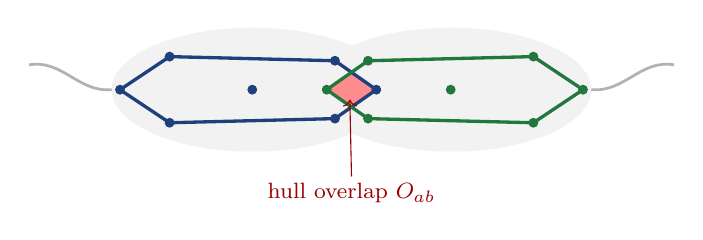
\begin{tikzpicture}[scale=1.05]
    % faint true silhouettes, for reference only
    \fill[gray!10] \bodyA;  \fill[gray!10] \bodyB;  \tails
    % hull intersection (the measured overlap)
    \begin{scope}\clip \hullA; \fill[red!45] \hullB; \end{scope}
    % the two hulls
    \draw[navy,very thick] \hullA;   \draw[forest,very thick] \hullB;
    % keypoints
    \foreach \p in {(1.5,0),(1.0,0.35),(1.0,-0.35),(0,0),(-1.0,0.4),(-1.0,-0.4),(-1.6,0)}
        \fill[navy] \p circle (1.7pt);
    \foreach \p in {(0.9,0),(1.4,0.35),(1.4,-0.35),(2.4,0),(3.4,0.4),(3.4,-0.4),(4.0,0)}
        \fill[forest] \p circle (1.7pt);
    \node[red!60!black] at (1.2,-1.25) {\footnotesize hull overlap $O_{ab}$};
    \draw[red!60!black,->] (1.2,-1.05) -- (1.18,-0.12);
  \end{tikzpicture}

  \vspace{0.2em}
  \footnotesize
  Convex hull $H_i=\mathrm{conv}(K_i)$ over each mouse's \textbf{12 keypoints} (dots).
  Contact $=$ polygon overlap
  $\;O_{ab}=\dfrac{\lvert H_a\cap H_b\rvert}{\lvert H_a\cup H_b\rvert}\;$ (red). Cheap, but
  built from \emph{sparse points}.
\end{frame}

% ----------------------------------------------- the weakness of hulls
\begin{frame}{Why hulls are weakest \emph{exactly during contact}}
  \begin{columns}[T]
    \begin{column}{0.54\textwidth}
      \begin{itemize}
        \item In close contact the \textbf{keypoints occlude} one another.
        \item On three \textbf{near-identical mice} the tracker \textbf{swaps / hallucinates}
              points.
        \item A polygon over a few noisy points \textbf{smooths over the true contact boundary}.
      \end{itemize}
      \vspace{0.4em}
      \begin{block}{The crux}
        The representation is \textbf{crudest at the very moment} the behaviour is defined.
      \end{block}
    \end{column}
    \begin{column}{0.44\textwidth}
      \centering
      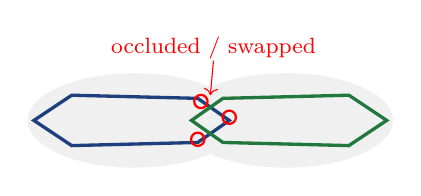
\begin{tikzpicture}[scale=0.8]
        \fill[gray!12] \bodyA; \fill[gray!12] \bodyB;
        \draw[navy,very thick] \hullA; \draw[forest,very thick] \hullB;
        % occluded / mislocated keypoints near the contact (jittered, red ring)
        \foreach \p in {(1.5,0.05),(1.05,0.30),(1.0,-0.30)}
            \draw[red,thick] \p circle (3pt);
        \node[red] at (1.25,1.15) {\footnotesize occluded / swapped};
        \draw[red,->] (1.25,0.95) -- (1.2,0.4);
      \end{tikzpicture}
    \end{column}
  \end{columns}
\end{frame}

% ---------------------------------------------------- principle 2: mask
\begin{frame}{Principle 2 — Mask contact geometry \small(our proposal, via SAM\,2)}
  \centering
  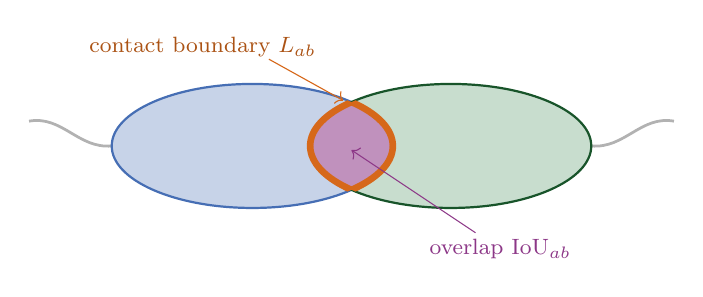
\begin{tikzpicture}[scale=1.05]
    % filled silhouettes (the masks)
    \fill[maskblue!30] \bodyA;  \fill[forest!25] \bodyB;  \tails
    % overlap = IoU region
    \begin{scope}\clip \bodyA; \fill[plum!55] \bodyB; \end{scope}
    % outlines
    \draw[maskblue,thick] \bodyA;  \draw[forest!70!black,thick] \bodyB;
    % contact boundary = each mask's outline that lies inside the other (orange)
    \begin{scope}\clip \bodyB; \draw[burnt,line width=2.4pt] \bodyA; \end{scope}
    \begin{scope}\clip \bodyA; \draw[burnt,line width=2.4pt] \bodyB; \end{scope}
    \node[plum]  at (3.0,-1.25) {\footnotesize overlap $\mathrm{IoU}_{ab}$};
    \draw[plum,->] (2.7,-1.05) -- (1.2,-0.05);
    \node[burnt!80!black] at (-0.6,1.2) {\footnotesize contact boundary $L_{ab}$};
    \draw[burnt,->] (0.2,1.05) -- (1.1,0.55);
  \end{tikzpicture}

  \vspace{0.2em}
  \footnotesize
  Full silhouettes $M_a,M_b$ (SAM\,2, prompted by the same keypoints).
  $\;\mathrm{IoU}_{ab}=\dfrac{\lvert M_a\cap M_b\rvert}{\lvert M_a\cup M_b\rvert}$ (plum) and
  \textbf{contact-boundary length} $L_{ab}=\lvert\partial M_a\cap(M_b\oplus B_r)\rvert$ (orange):
  \emph{how much of the two silhouettes physically touch}.
\end{frame}

% ------------------------------------------------------- the bet, side by side
\begin{frame}{The bet: same contact, two measurements}
  \begin{columns}[T]
    \begin{column}{0.5\textwidth}
      \centering\textbf{\color{navy}Hull} — sparse points
      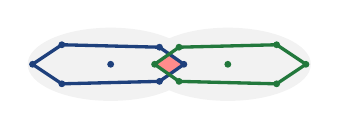
\begin{tikzpicture}[scale=0.62]
        \fill[gray!10] \bodyA; \fill[gray!10] \bodyB;
        \begin{scope}\clip \hullA; \fill[red!45] \hullB; \end{scope}
        \draw[navy,very thick] \hullA; \draw[forest,very thick] \hullB;
        \foreach \p in {(1.5,0),(1.0,0.35),(1.0,-0.35),(-1.0,0.4),(-1.0,-0.4),(-1.6,0),(0,0)}
            \fill[navy] \p circle (2pt);
        \foreach \p in {(0.9,0),(1.4,0.35),(1.4,-0.35),(3.4,0.4),(3.4,-0.4),(4.0,0),(2.4,0)}
            \fill[forest] \p circle (2pt);
      \end{tikzpicture}\\[2pt]
      \footnotesize\color{red!60!black}\textbf{under-reads} the contact
    \end{column}
    \begin{column}{0.5\textwidth}
      \centering\textbf{\color{maskblue}Mask} — full silhouette
      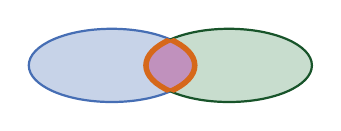
\begin{tikzpicture}[scale=0.62]
        \fill[maskblue!30] \bodyA; \fill[forest!25] \bodyB;
        \begin{scope}\clip \bodyA; \fill[plum!55] \bodyB; \end{scope}
        \draw[maskblue,thick] \bodyA; \draw[forest!70!black,thick] \bodyB;
        \begin{scope}\clip \bodyB; \draw[burnt,line width=2pt] \bodyA; \end{scope}
        \begin{scope}\clip \bodyA; \draw[burnt,line width=2pt] \bodyB; \end{scope}
      \end{tikzpicture}\\[2pt]
      \footnotesize\color{forest!60!black}\textbf{sees} the real overlap $+$ boundary
    \end{column}
  \end{columns}
  \vspace{0.5em}
  \centering\small
  Both start from the \textbf{same keypoints} $\Rightarrow$ the comparison isolates the
  \emph{representation}, not the pose. \textbf{Hypothesis:} the gap is largest on the
  deepest-contact behaviours.
\end{frame}

% ----------------------------------------------------------- the pipeline
\begin{frame}{How it runs: everything heavy is frozen \& cached}
  \centering
  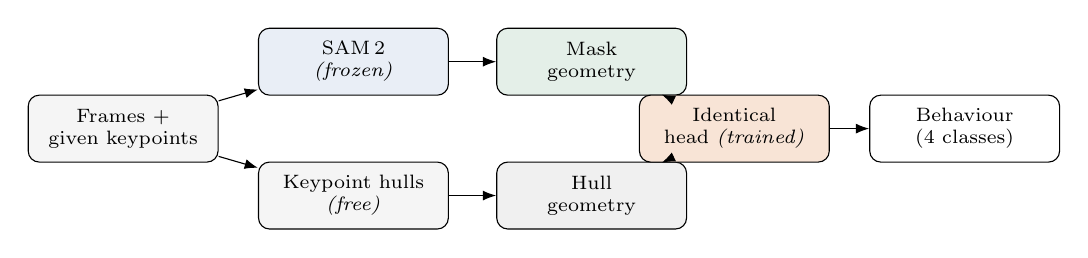
\begin{tikzpicture}[>=Latex,
    box/.style={draw,rounded corners,align=center,font=\scriptsize,inner sep=3pt,
                minimum height=0.85cm,text width=2.2cm}]
    \node[box,fill=black!4] (in) {Frames $+$\\given keypoints};
    \node[box,fill=maskblue!12,right=0.5cm of in,yshift=0.85cm] (sam) {SAM\,2\\\textit{(frozen)}};
    \node[box,fill=black!4,right=0.5cm of in,yshift=-0.85cm] (hull) {Keypoint hulls\\\textit{(free)}};
    \node[box,fill=forest!12,right=0.6cm of sam] (mgeo) {Mask\\geometry};
    \node[box,fill=black!6,right=0.6cm of hull] (hgeo) {Hull\\geometry};
    \node[box,fill=burnt!18,right=0.6cm of $(mgeo)!0.5!(hgeo)$] (head) {Identical\\head \textit{(trained)}};
    \node[box,right=0.5cm of head] (out) {Behaviour\\(4 classes)};
    \draw[->] (in)--(sam); \draw[->] (in)--(hull);
    \draw[->] (sam)--(mgeo); \draw[->] (hull)--(hgeo);
    \draw[->] (mgeo)--(head); \draw[->] (hgeo)--(head); \draw[->] (head)--(out);
  \end{tikzpicture}

  \vspace{0.6em}
  \footnotesize
  SAM\,2 \& VideoMAE are \textbf{inference-only}; features cached once. The \textbf{only} trained
  part is a small head of \textbf{identical capacity} in every condition — so a gain reflects
  \emph{information, not parameters}.
\end{frame}

% ------------------------------------------------------------------ data
\begin{frame}{The data: MABe22 mouse-triplet}
  \begin{columns}[T]
    \begin{column}{0.56\textwidth}
      \begin{itemize}
        \item \textbf{1{,}830} labelled 1-min sequences @ 30\,Hz (224$\times$224 top-view).
        \item \textbf{3 near-identical mice}, \textbf{12 given keypoints} each.
        \item \textbf{Dense framewise labels} for four behaviours.
        \item Top-view lab mice $=$ easy \emph{imaging}; the hard part is \emph{identity through
              contact}.
      \end{itemize}
    \end{column}
    \begin{column}{0.44\textwidth}
      \footnotesize
      \begin{tabular}{@{}lr@{}}
        \textbf{Behaviour} & \textbf{positive} \\\hline
        \texttt{huddles}              & 8.1\,\% \\
        \texttt{oral\_oral\_contact}  & 0.23\,\% \\
        \texttt{oral\_genital\_contact} & 0.23\,\% \\
        \texttt{chases}               & 0.05\,\% \\
      \end{tabular}
      \vspace{0.4em}\\
      Heavy imbalance $\Rightarrow$ report \textbf{AP} as well as F1.
    \end{column}
  \end{columns}
  \vspace{0.4em}
  \footnotesize\textbf{Eval contract (already locked):} framewise, four independent binary tasks;
  \textbf{leakage-safe split by sequence}; per-behaviour F1 $+$ AP, macro-averaged.
\end{frame}

% ----------------------------------------------------- experiment / ablations
\begin{frame}{The experiment (pre-registered)}
  \begin{enumerate}
    \item[\textbf{a}] \textbf{Hull geometry} alone — the baseline.
    \item[\textbf{b}] \textbf{Mask geometry} alone \;vs\; (a) — \textcolor{burnt}{\textbf{the key
          head-to-head}}.
    \item[\textbf{c}] \textbf{Fusion}: mask geometry on top of frozen VideoMAE — does it add over
          what VideoMAE already sees?
  \end{enumerate}
  \vspace{0.4em}
  \begin{itemize}
    \item Identical head capacity; $\geq 5$ seeds; mean $\pm$ 95\,\% CI; per-behaviour scores.
    \item \textbf{Success fixed up front:} mask beats hull with a CI excluding zero \emph{and} a
          pre-set minimum effect, \emph{or} a clear win on the deepest-contact behaviours.
    \item Scrambled-mask control rules out a capacity artefact.
  \end{itemize}
  \begin{block}{}
    \centering Interpretable \textbf{either direction} — a clean negative is still a result.
  \end{block}
\end{frame}

% ------------------------------------------------------------- the one risk
\begin{frame}{The one make-or-break risk (settled in week 1)}
  \centering\small
  \emph{Can SAM\,2 keep three near-identical mice separate \& identity-stable
  \textbf{through the contact frames}?}
  \vspace{0.5em}
  \begin{columns}[T]
    \begin{column}{0.32\textwidth}
      \begin{block}{\small PASS}
        \footnotesize identities hold $\rightarrow$ proceed; contact geometry is the headline.
      \end{block}
    \end{column}
    \begin{column}{0.34\textwidth}
      \begin{block}{\small PARTIAL}
        \footnotesize masks merge only in deepest contact $\rightarrow$ use the
        \emph{merge event itself} as a coarse high-contact feature.
      \end{block}
    \end{column}
    \begin{column}{0.32\textwidth}
      \begin{block}{\small FAIL}
        \footnotesize frequent swaps $\rightarrow$ pivot headline to \textbf{background-robustness},
        report this as a negative result.
      \end{block}
    \end{column}
  \end{columns}
  \vspace{0.5em}
  A \textbf{week-1 masking pilot} on huddle/chase clips fires this decision. The dissertation keeps
  a clean spine either way.
\end{frame}

% ------------------------------------------------------------- timeline
\begin{frame}{Eight-week plan}
  \footnotesize
  \begin{tabular}{@{}rl@{}}
    \textbf{Wk 1} & Acquire $+$ lock eval contract \;\textcolor{forest}{(done)}; \textbf{masking pilot $+$ decision}.\\
    \textbf{Wk 2} & Scoped SAM\,2 mask cache (Kaggle); begin geometry features.\\
    \textbf{Wk 3} & Finish contact-geometry $+$ hull extractor; head overfit sanity.\\
    \textbf{Wk 4} & \textbf{Mask vs hull head-to-head} — first real result.\\
    \textbf{Wk 5} & Per-behaviour analysis; multi-seed CIs; go/no-go on MammAlps.\\
    \textbf{Wk 6} & Fusion / VideoMAE-redundancy test; lock primary.\\
    \textbf{Wk 7} & Background-shift robustness (insurance); consolidate.\\
    \textbf{Wk 8} & Write-up; figures; package pipeline $+$ code.\\
  \end{tabular}
  \vspace{0.4em}\\
  All risk front-loaded into week 1; the headline result by week 4.
\end{frame}

% ------------------------------------------------------------- takeaway
\begin{frame}{Contribution}
  \begin{block}{}
    \centering To our knowledge, the \textbf{first use of inter-animal segmentation-mask contact
    geometry} (mask IoU, contact-boundary length) as an explicit feature for social-behaviour
    recognition — in a clean head-to-head against the keypoint-hull geometry the field already
    uses.
  \end{block}
  \vspace{0.3em}
  \begin{itemize}
    \item Honest framing: shape-from-silhouette is \emph{not} new; the \textbf{mask-contact
          measurement} and the \textbf{controlled comparison} are.
    \item Every heavy model frozen; reproducible from cache; multi-seed CIs.
    \item Built-in insurance: background-robustness if the masking pilot fails.
  \end{itemize}
  \vspace{0.4em}
  \centering\small\color{navy}\textbf{Thank you — questions welcome.}
\end{frame}

\end{document}
